% $Id: LD2004.tex,v 1.3 2005/02/03 05:55:49 doros Exp $

% This program can be redistributed and/or modified under the terms
% of the Creative Common Licence

\documentclass{beamer}

%\usepackage[headheight=12pt]{beamerthemeboxes}
%\usepackage{beamerthemesplit}
%\usepackage{graphics}

\beamertemplateshadingbackground{red!10}{blue!10}

\usepackage{beamerthemeshadow}

\usepackage[italian]{babel}
%\usepackage{pgf,pgfarrows,pgfnodes,pgfautomata,pgfheaps}
%\usepackage{amsmath,amssymb}
%\usepackage[latin1]{inputenc}
%\usepackage{times}
\usepackage{palatino}

\usepackage{hyperref}

% Use some nice templates

\beamertemplateshadingbackground{red!10}{structure!10}
\beamertemplatetransparentcovereddynamic
\beamertemplateballitem
\beamertemplatenumberedballsectiontoc






%\title{Netkit4TIC: il laboratorio virtuale per lo studio di reti e di servizi di rete}
\title{Netkit4TIC: il laboratorio virtuale per lo studio di reti}
\author{Sandro Doro}
\institute[ITIS "C.Zuccante" - Venezia--Mestre]{
  ITIS "C.Zuccante" - Venezia--Mestre\\
  Corso Serale Sirio}
%       Linux registered user n. 5768
%\date{\today}
\date{LinuxDay 2004}

\AtBeginSection[]{\frame{\frametitle{Programma}\tableofcontents[current]}}



\pgfdeclaremask{tu}{uml-small-mask}
\pgfdeclareimage[mask=tu,width=1cm]{tu-logo}{uml-small}

\logo{\pgfuseimage{tu-logo}}



\begin{document}

%\frame{\maketitle}
\frame{\titlepage
%  \footnotetext{Prodotto con \LaTeX e pdf\LaTeX}
}

\section*{Programma}
\frame{\frametitle{Programma}\tableofcontents[part=1]}



\part{Main part}

%\frame{\partpage}

\section{Gli ambienti virtuali}
\frame{
  \frametitle{Gli ambienti virtuali}
  \begin{block}{Osservazione}
  Da alcuni anni si stanno diffondendo progetti il cui scopo \`{e}
  quello di simulare altri sistemi, sia hardware che software.

  La virtualizzazione di una intera macchina apre nuovi
  scenari nella sperimentazione con il software.\\
  Questa idea non \`{e} nuova poich\`{e}
  risale all'epoca d'oro dei mainframe.
  \end{block}

}
\subsection{UML}
\frame{
  \frametitle{User Mode Linux}
  \begin{block}{http://www.user-mode-linux.org}
  \`{E} un progetto ospitato sul sito sourgeforge.net e il suo
  ideatore e autore \`{e} Jeff Dike.\\
  Contribuisce al progetto
  una vasta parte della comunit\`{a} open--source compreso un
  giovane italiano distintosi l'anno scorso
  alle Olimpiadi della matematica.
  \end{block}
}
\frame{
  \frametitle{User Mode Linux - caratteristiche}
  \begin{itemize}
    \item Permette di eseguire il kernel Linux in ambiente Linux ossia
          da un pc con installato GNU/Linux posso "creare" un altro
          sistema GNU/Linux anche con una diversa distribuzione.\\
          Dal ci\`{o} deriva che non si fa
          girare solo un programma ma un intero sistema.
    \item \`{E} un sistema di virtualizzazione (chiamato anche di simulazione)
  \end{itemize}
}
\frame{
  \frametitle{User Mode Linux - come lavora}
          Normalmente un programma che necessita dell'uso dell'hardware
          (scheda video, tastiera, ecc) deve richiedere il servizio
          al kernel.\\
          Nel caso di utilizzo del sistema UML la richiesta viene
          fatta al kernel UML.
  %\center{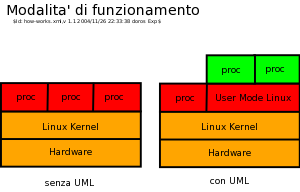
\includegraphics[height=4cm]{how-works.png}}
  \begin{center}
  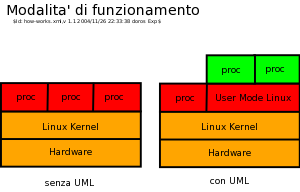
\includegraphics[width=7cm]{how-works.png}
  \end{center}
}
\subsection{Applicazioni}
\frame{
  \frametitle{Applicazioni}
  I contesti in cui si utilizza la virtualizzazione di un intero sistema
  operativo sono ad esempio:

  \begin{itemize}
    \item Ambiente di testing di nuovo software
    \item Ambiente di simulazione di protocolli di rete
    \item Costruzione di Honeynet virtuali
    \item Costruzione di Virtual Host per Hosting Service
    \item Costruzione di Virtual Cluster con OpenMosix
  \end{itemize}
}
\frame{
  \label{test}
  \frametitle{UML - Ambiente di testing di nuovo software}
  Il progetto FreeSWAN (IPsec per Linux):
  \begin{itemize}
    \item si basa su righe di codice
  estremamente complicate per la comunicazione in rete
    \item cifra tutto il traffico di rete
    \item Utilizza un sistema
  di chiavi dinamico che rende praticamente impossibile ad un osservatore
  di capire cosa viene trasmesso
    \item occorrono circa 6
  sistemi per testare completamente il codice prodotto e quindi \`{e}
  impossibile o troppo costoso tenere un tale sistema dispobile
  solo per questo scopo
  \end{itemize}
}
\frame{
  \label{simu}
  \frametitle{Ambiente di sperimentazione di protocolli di rete}
  Il progetto UMTS/TIC corsi C1 e C2 \`{e} stato un progetto del MIUR
  per la formazione del personale interno (ATA e docenti) sulla
  infrastruttura tecnologica.\\
  Si sono verificati alcuni problemi:
  \begin{itemize}
    \item mancanza di un laboratorio creato appositamente e sempre accessibile
    ai corsisti per effettuare le loro prove
    \item mancanza di un sufficiente numero di computer
    \item impossibilit\`{a} di effettuare le esercitazioni a casa
  \end{itemize}
}
\frame{
  \frametitle{Laboratorio di sistemi/informatica}
  Negli istituti tecnici a indirizzo informatica (ABACUS/Sirio)
  nell'ultimo anno di corso, a volte anche prima, si studiano
  le reti e le applicazioni web. Per l'assimilizione effettiva
  da parte degli studenti sarebbe opportuno:
  \begin{itemize}
    \item mettere a disposizione \textbf{per ogni studente} un gruppo di sistemi
          da configurare e amministrare
    \item avere lo stesso sistema a casa
  \end{itemize}
}
\frame{
  \frametitle{Costruzione di Honeynet (vasi di miele)}
  Gli Honeynet sono dei sistemi installati sulle reti e servono per attirare
  eventuali intrusi e per studiare le loro mosse.
  Queste reti
  di sistemi sono altamente controllate e quando uno dei sistemi
  \`{e} attaccato esso cattura tutta l'attivit\`{a} dell'intruso.
  Un articolo che spiega come costruirli \`{e}:
  \href{http://www.honeynet.org/papers/virtual/}{"Know Your Enemy: Defining Virtual Honeynets"}
  tradotti in italiano in una serie di tre articoli(
  \href{http://www.honeynet.org/papers/trans/nemico.html}{1},
  \href{http://www.honeynet.org/papers/trans/nemico2.html}{2},
  \href{http://www.honeynet.org/papers/trans/nemico3.html}{3})
}
\frame{
  \frametitle{Costruzione di Virtual Host per Hosting Service}
  La vendita di servizi di hosting \`{e} un mercato in forte crescita
  e spesso chi li utilizza desidera passare dalla soluzione
  di delega della gestione dei propri servizi al pieno possesso
  degli stessi per ottenere pi\`{u} flessibilit\`{a}.
  La soluzione pi\`{u} vantaggiosa \`{e} sicuramente l'acquisto
  di un sistema virtuale.
  Un articolo che racconta la nascita di un provider di questo tipo \`{e}:
  \href{http://uml.openconsultancy.com/}{"UML-based pseudo-dedicated hosting service"}
}
\frame{
  \begin{center}
  
\includegraphics[width=3cm]{OpenMosix.jpg}
  \end{center}
  \frametitle{Costruzione di Cluster con OpenMosix}
  OpenMosix \`{e} un progetto Open Source che estende il
  kernel di Linux per costruire cluster basati su una
  singola immagine. Una fotografia di un cluser \`{e} visibile sullo
  \href{http://www.mosixview.com/umopenmosix/umopenmosix.jpg}{screenshot}.
  Un articolo che descrive come costruire un cluster UML OpenMosix \`{e}:
  \href{http://www.mosixview.com/umopenmosix/umopenmosix.html}{"User Mode openMosix: a virtual openMosix cluster running in User-mode"}
}





\section{Netkit}
\frame{
  \frametitle{Cos'\`{e} Netkit - http://www.netkit.org}
    Netkit \`{e} il risultato del lavoro di alcune persone del
    Networks Research Group dell'Universit\`{a} di Roma 3 e
    del Linux User Group LUG Roma 3. Il software \`{e} composto da:
  \begin{itemize}
    \item Un insieme predefinito di comandi per il setup di
          macchine virtuali
    \item Un filesystem con preinstallato il software
          necessario per le sperimentazioni
  \end{itemize}
}
\subsection{Linee guida}
\frame{
  \frametitle{Linee guida}
  Netkit \`{e} stato concepito come un ambiente a basso costo per
  esperimenti di rete. All'interno del suo ambiente possono essere
  "creati" e interconessi dei completi router, switch e host. Tali
  apparati sono virtuali ma possono operare con molte delle
  caratteristiche possedute da quelli reali.
}
\subsection{Informazioni generali}
\frame{
  \frametitle{Considerazioni generali}
  \begin{itemize}
    \item Basato su User Mode Linux
    \item Ogni apparato di rete \`{e} una linux box
    \item Linux supporta quasi tutti i protocolli di rete
          e pu\`{o} essere configurato come bridge/switch o
          come router
  \end{itemize}
}
\subsection{Struttura}
\frame{
  \frametitle{Struttura}
  \begin{itemize}
    \item Le varie istanze che simulano gli apparati di rete
          sono create all'interno dello stesso host
    \item Le varie istanze sono interconnesse in domini di
          collisione (hub/switch)
    \item Il ruoli dei nodi sono configurabili
  \end{itemize}
}
\subsection{Esperienze sperimentabili}
\frame{
  \frametitle{Esperienze sperimentabili}
  \begin{itemize}
    \item Esperienze base: rete minimale con due host, tabelle di routing,
          protocollo ARP, protocollo RIP.
    \item Esperienze applicative: configurazione di DNS e Mail server.
    \item Esperienze avanzate: esperienze su switch e STP.
    \item Esperienze su routing interdomio (bgp): routing tra Autonomous
          System.
  \end{itemize}
}




\section{Netkit4TIC}
\frame{
  \frametitle{Netkit4TIC - http://www.tic.fdns.net/tic/html/lab.html}
  Questo progetto \`{e} nato nel 2002 dalla necessit\`{a} nei
  corsi UMTS/TIC C2 di un laboratorio
  di sperimentazione "permanente".\\
  Le aree di interesse, intersecate tra loro, si possono
  dividere in:
  \begin{itemize}
    \item problematiche di rete: lo stack TCP/IP e la
          progettazione in generale di reti
    \item configurazione servizi: Web, DNS, 
          directory services, file share, Kerberos, Terminal Server
    \item problematiche sulla sicurezza: cifratura,
          certificati elettronici, VPN
  \end{itemize}
}
\subsection{Struttura}
\frame{
  \frametitle{Struttura}
  \`{E} composto da una prima parte statica
  e corposa e da una seconda parte dinamica ed esile:
  \begin{enumerate}
    \item Live CD: \`{e} una distribuzione GNU/Linux in grado di
          "eseguire" le esperienze senza bisogno di installazione. Contiene:
    \begin{itemize}
      \item una versione di Knoppix elaborata per ottenere migliori
            prestazioni con UML.
      \item un filesystem e un kernel per UML allineato alla distribuzione
            GNU/Linux Debian sarge
      \item un filesystem per UML per il firewall LEAF/Bering con
            librerie uClibc per sistemi embeded.
      \item una versione personalizzata di Netkit
    \end{itemize}
    \item Internet: dal sito
          \href{http://www.tic.fdns.net/tic/html/lab.html}{http://www.tic.fdns.net/tic/html/lab.html}
          sono scaricabili le esperienze virtuali (qualche Kbyte) in formato archivio compresso (tgz).
  \end{enumerate}
}
\subsection{Esperienze sperimentabili}
\frame{
  \frametitle{lo stack TCP/IP e la progettazione di reti}
  \begin{block}{Esperienze sperimentabili}
  \begin{itemize}
    \item bridge, Bridge+STP, VLAN, proxyARP
    \item tabella di routing (statica), protocollo OSPF, Controllo LAB
    \item Qualit\`{a} del Servizio (QoS)
    \item Esercizi: NetPractice
  \end{itemize}
  \end{block}
}
\frame{
  \frametitle{Web, DNS, directory services, Kerberos, file share, LTSP}
  \begin{block}{Esperienze sperimentabili}
  \begin{itemize}
    \item file sharing: Samba + Samba Enterprise
    \item directory service: OpenLDAP
    \item Kerberos V
    \item Terminal Server
    \item Manutenzione reti via SNMP
  \end{itemize}
  \end{block}
}
\frame{
  \frametitle{Sicurezza}
  \begin{block}{Esperienze sperimentabili}
  \begin{itemize}
    \item Firewall
    \begin{itemize}
       \item a singola area interna
       \item con area interna e area smilitarizzata (DMZ)
       \item con due are perimetrali e backbone interno
    \end{itemize}
    \item PKI: OpenCA una infrastruttura Open Source 
    \item Protocolli SSH e SSL
    \item VPN
    \item Sistemi di rilevazione intrusioni
  \end{itemize}
  \end{block}
}
\subsection{Demo}
\frame{
  \frametitle{Virtual PHP-Nuke}
  \begin{block}{Esperienza sul portale virtuale}
  \begin{center}
  
\includegraphics[width=8cm]{PHP-Nuke.png}
  \end{center}
  \end{block}
}
\frame[containsverbatim]{
  \frametitle{Virtual PHP-Nuke}
  \begin{block}{script esperienza Netkit4TIC}
  \footnotesize
  \begin{verbatim}
$ wget http://www.tic.fdns.net/tic/html/PHP-Nuke.tgz
$ tar zxf PHP-Nuke.tgz
$ cd php
$ tunctl
$ sudo su

# ifconfig tap0 192.168.77.2
# echo "1" > /proc/sys/net/ipv4/ip_forward
# exit

$ ./lab start
$ mozilla http://192.168.77.1/
  \end{verbatim}
  \end{block}
}

\section*{Sommario}

\frame{
  \frametitle{Sommario}

  \begin{block}{Riassunto}
  \begin{itemize}
  \item
    Lo studio e la progettazione di reti e di servizi di rete \`{e} un
    elemento essenziale del nostro futuro.
  \item
    La modalit\`{a} dell'apprendimento virtuale \`{e} in grande
    espansione.
  \item
    Esiste una via economica e valida: Netkit4TIC
  \end{itemize}
  \end{block}{}

  \begin{block}{Problemi Aperti}
    \begin{itemize}
    \item
      Adozione
    \item
      Documentazione dettagliata e di qualit\`{a} anche in lingua inglese.
    \end{itemize}
  \end{block}


}

%\frame{}   % to enforce entries in the table of contents

\end{document}
